\documentclass{article}\usepackage[]{graphicx}\usepackage[]{color}
%% maxwidth is the original width if it is less than linewidth
%% otherwise use linewidth (to make sure the graphics do not exceed the margin)
\makeatletter
\def\maxwidth{ %
  \ifdim\Gin@nat@width>\linewidth
    \linewidth
  \else
    \Gin@nat@width
  \fi
}
\makeatother

\definecolor{fgcolor}{rgb}{0.345, 0.345, 0.345}
\newcommand{\hlnum}[1]{\textcolor[rgb]{0.686,0.059,0.569}{#1}}%
\newcommand{\hlstr}[1]{\textcolor[rgb]{0.192,0.494,0.8}{#1}}%
\newcommand{\hlcom}[1]{\textcolor[rgb]{0.678,0.584,0.686}{\textit{#1}}}%
\newcommand{\hlopt}[1]{\textcolor[rgb]{0,0,0}{#1}}%
\newcommand{\hlstd}[1]{\textcolor[rgb]{0.345,0.345,0.345}{#1}}%
\newcommand{\hlkwa}[1]{\textcolor[rgb]{0.161,0.373,0.58}{\textbf{#1}}}%
\newcommand{\hlkwb}[1]{\textcolor[rgb]{0.69,0.353,0.396}{#1}}%
\newcommand{\hlkwc}[1]{\textcolor[rgb]{0.333,0.667,0.333}{#1}}%
\newcommand{\hlkwd}[1]{\textcolor[rgb]{0.737,0.353,0.396}{\textbf{#1}}}%
\let\hlipl\hlkwb

\usepackage{framed}
\makeatletter
\newenvironment{kframe}{%
 \def\at@end@of@kframe{}%
 \ifinner\ifhmode%
  \def\at@end@of@kframe{\end{minipage}}%
  \begin{minipage}{\columnwidth}%
 \fi\fi%
 \def\FrameCommand##1{\hskip\@totalleftmargin \hskip-\fboxsep
 \colorbox{shadecolor}{##1}\hskip-\fboxsep
     % There is no \\@totalrightmargin, so:
     \hskip-\linewidth \hskip-\@totalleftmargin \hskip\columnwidth}%
 \MakeFramed {\advance\hsize-\width
   \@totalleftmargin\z@ \linewidth\hsize
   \@setminipage}}%
 {\par\unskip\endMakeFramed%
 \at@end@of@kframe}
\makeatother

\definecolor{shadecolor}{rgb}{.97, .97, .97}
\definecolor{messagecolor}{rgb}{0, 0, 0}
\definecolor{warningcolor}{rgb}{1, 0, 1}
\definecolor{errorcolor}{rgb}{1, 0, 0}
\newenvironment{knitrout}{}{} % an empty environment to be redefined in TeX

\usepackage{alltt}

\usepackage{fancyhdr} % Required for custom headers
\usepackage{lastpage} % Required to determine the last page for the footer
\usepackage{extramarks} % Required for headers and footers
\usepackage{graphicx} % Required to insert images
\usepackage{hyperref}
\usepackage{amsmath} %for binomial pdf
\usepackage{parskip} % so that there's space bw paragraphs
\usepackage{float}
\usepackage{amsfonts}
\graphicspath{"~/almhub_0823/exp_design/homework/HW4"}



% Margins
\topmargin=-0.45in
\evensidemargin=0in
\oddsidemargin=0in
\textwidth=6.5in
\textheight=9.0in
\headsep=0.25in 

\linespread{1.1} % Line spacing

% Set up the header and footer
\pagestyle{fancy}
\lhead{STAT 541: Experimental Design} % Top left header
\chead{HW 3} % Top center header
\rhead{Andrea Mack} % Top right header
\lfoot{02/10/2017} % Bottom left footer
\cfoot{} % Bottom center footer
\rfoot{Page\ \thepage\ of\ \pageref{LastPage}} % Bottom right footer
\renewcommand\headrulewidth{0.4pt} % Size of the header rule
\renewcommand\footrulewidth{0.4pt} % Size of the footer rule

\setlength\parindent{0pt} % Removes all indentation from paragraphs
\setlength\parskip{0.5cm}
\restylefloat{table}

%----------------------------------------------------------------------------------------
%	DOCUMENT STRUCTURE COMMANDS
%	Skip this unless you know what you're doing
%----------------------------------------------------------------------------------------

% Header and footer for when a page split occurs within a problem environment
\newcommand{\enterProblemHeader}[1]{
\nobreak\extramarks{#1}{#1 continued on next page\ldots}\nobreak
\nobreak\extramarks{#1 (continued)}{#1 continued on next page\ldots}\nobreak
}

% Header and footer for when a page split occurs between problem environments
\newcommand{\exitProblemHeader}[1]{
\nobreak\extramarks{#1 (continued)}{#1 continued on next page\ldots}\nobreak
\nobreak\extramarks{#1}{}\nobreak
}


%----------------------------------------------------------------------------------------%
\IfFileExists{upquote.sty}{\usepackage{upquote}}{}
\begin{document}



\begin{enumerate}
        
\item %1

Hand written.

\item %2

Hand written.

\item %3
\begin{enumerate}
\item %3a

$H_{0}$: $\sigma^{2}_{batch} = 0$

$H_{A}$: $\sigma^{2}_{batch} > 0$

Based on an $F_{4,20}$ statistic of 5.54 and p-value of $<$ 0.0036 there is strong evidence of batch to batch variation.

\begin{knitrout}\footnotesize
\definecolor{shadecolor}{rgb}{0.969, 0.969, 0.969}\color{fgcolor}\begin{kframe}
\begin{alltt}
\hlstd{chi.cutL} \hlkwb{<-} \hlkwd{pchisq}\hlstd{(}\hlnum{0.025}\hlstd{,}\hlnum{20}\hlstd{,} \hlkwc{lower.tail} \hlstd{=} \hlnum{TRUE}\hlstd{)}
\hlstd{chi.cutU} \hlkwb{<-} \hlkwd{pchisq}\hlstd{(}\hlnum{0.975}\hlstd{,}\hlnum{20}\hlstd{,} \hlkwc{lower.tail} \hlstd{=} \hlnum{TRUE}\hlstd{)}

\hlstd{sigma2} \hlkwb{<-} \hlnum{0.00483}
\hlstd{sse} \hlkwb{<-} \hlnum{0.0876}

\hlstd{ll} \hlkwb{<-} \hlstd{sse}\hlopt{/}\hlstd{chi.cutL}
\hlstd{ul} \hlkwb{<-} \hlstd{sse}\hlopt{/}\hlstd{chi.cutU}

\hlstd{ci} \hlkwb{<-} \hlkwd{c}\hlstd{(sigma2}\hlopt{-}\hlstd{ll,sigma2}\hlopt{+}\hlstd{ul)}
\end{alltt}
\end{kframe}
\end{knitrout}

$\sigma^{2}$ was estimated to be 0.00438 and the approximate 95\% confidence interval is between \Sepr{ci[1]} and \ensuremath{6.5257365\times 10^{8}}. That is, the within batch variation calcium content is estimated to be between \Sepr{ci[1]} and \ensuremath{6.5257365\times 10^{8}} at the 95\% confidence level. 

Note that $\sigma^{2}$ must be positive, but the confidence interval given includes negative values.

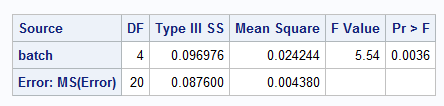
\includegraphics{prob3tb}



\item %3b

$\hat{\sigma^{2}}_{batch}$ = $MS_{batch}$ = 0.024244

$\hat{\sigma^{2}}$ = $MS_{error}$ = 0.00438

$\hat{\sigma^{2}}_{t}$ = $\frac{MS_{batch} - MS_{error}}{5}$ = 0.0038812

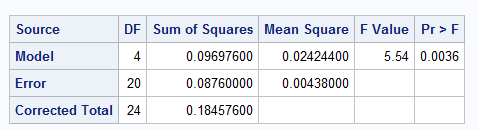
\includegraphics{prob3ss}

\item %3c

\begin{knitrout}\footnotesize
\definecolor{shadecolor}{rgb}{0.969, 0.969, 0.969}\color{fgcolor}\begin{kframe}
\begin{alltt}
\hlstd{F0L} \hlkwb{<-} \hlkwd{pchisq}\hlstd{(}\hlnum{0.025}\hlstd{,}\hlnum{5}\hlstd{,} \hlkwc{lower.tail} \hlstd{=} \hlnum{TRUE}\hlstd{)}
\hlstd{F0U} \hlkwb{<-} \hlkwd{pchisq}\hlstd{(}\hlnum{0.975}\hlstd{,}\hlnum{5}\hlstd{,}\hlkwc{lower.tail} \hlstd{=} \hlnum{TRUE}\hlstd{)}

\hlstd{FL} \hlkwb{<-} \hlkwd{qf}\hlstd{(}\hlnum{0.025}\hlstd{,}\hlnum{4}\hlstd{,}\hlnum{20}\hlstd{)}
\hlstd{FU} \hlkwb{<-} \hlkwd{qf}\hlstd{(}\hlnum{0.975}\hlstd{,}\hlnum{4}\hlstd{,}\hlnum{20}\hlstd{)}


\hlstd{chi.cutL4} \hlkwb{<-} \hlkwd{qchisq}\hlstd{(}\hlnum{0.025}\hlstd{,}\hlnum{4}\hlstd{,} \hlkwc{lower.tail} \hlstd{=} \hlnum{TRUE}\hlstd{)}
\hlstd{chi.cutU4} \hlkwb{<-} \hlkwd{qchisq}\hlstd{(}\hlnum{0.975}\hlstd{,}\hlnum{4}\hlstd{,} \hlkwc{lower.tail} \hlstd{=} \hlnum{TRUE}\hlstd{)}

\hlstd{sigma2B} \hlkwb{<-} \hlnum{0.024244}
\hlstd{sst} \hlkwb{<-} \hlnum{0.09697600}

\hlstd{frac.s} \hlkwb{<-} \hlstd{sigma2B}\hlopt{/}\hlstd{(sigma2B} \hlopt{+} \hlstd{sigma2)}

\hlstd{llB} \hlkwb{<-} \hlstd{(sst}\hlopt{*}\hlstd{(}\hlnum{1}\hlopt{-}\hlstd{(FU}\hlopt{/}\hlstd{F0U)))}\hlopt{/}\hlnum{5}\hlopt{*}\hlstd{chi.cutL4}
\hlstd{ulB} \hlkwb{<-} \hlstd{(sst}\hlopt{*}\hlstd{(}\hlnum{1}\hlopt{-}\hlstd{(FL}\hlopt{/}\hlstd{F0L)))}\hlopt{/}\hlnum{5}\hlopt{*}\hlstd{chi.cutU4}

\hlstd{ciB} \hlkwb{<-} \hlkwd{c}\hlstd{(frac.s}\hlopt{-}\hlstd{llB,frac.s}\hlopt{+}\hlstd{ulB)}
\end{alltt}
\end{kframe}
\end{knitrout}

The percent of batch to batch variability relative to total variability was 0.8338722 with an estimated 95\% confidence interval of between 1.7561655 and -4845.290826 percent.



\item %3d

Although the problem said to do an ANOVA, I fit a random effects model.

It appears there is a slight violation of the normality assumption as the quantiles of the residuals show slight deviations than those expected under normality in the tails. This is not a major concern.

It is reasonable to assume the variation is the same within each batch as shown by the fitted vs. residuals plot.

The problem description said that batches were randomly chosen, which makes them independent.

The problem description did not say the ``five determinations" were randomly chosen, and so observations within each batch may not be independent of other observations in the same batch.

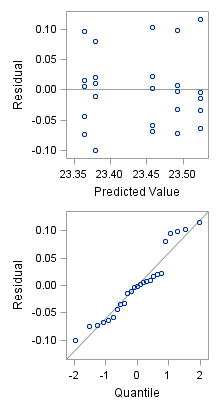
\includegraphics[scale=0.5]{prob3plots}


\end{enumerate}

\newpage

\item %4
\begin{enumerate}
\item %4a

{\bf MODEL}

$y = \mu + \tau_{1hr} + \tau_{2hr} + \tau_{4hr} + \epsilon$

y: BMD loss

$\mu$: The average BMD loss in the SHAM group

$\tau_{1hr}$: The change in average BMD loss between the SHAM group and the 1hr/day PEMF group

$\tau_{2hr}$: The change in average BMD loss between the SHAM group and the 2hr/day PEMF group

$\tau_{4hr}$: The change in average BMD loss between the SHAM group and the 4hr/day PEMF group

$\epsilon$: random error

{\bf ANOVA ASSUMPTIONS}

$\epsilon_{i} \sim iid N(0,\sigma^{2})$

The errors are independently and normally distributed with a mean of 0 and with the similar variance of $\sigma^{2}$.

\item %4b

Note that assuming $\Sigma \tau_{i}$ = 0 specifies the means model, which is a different parameterization than the effects model written in (a).


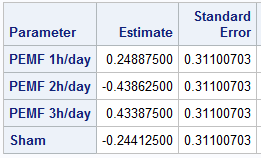
\includegraphics{estse4b}

\item %4c

With the Normal Q-Q plot we are assessing whether it is reasonable to assume the residuals are normally distributed. There is slight deviation from normality in the upper tail of the distribution, but for the most part it is reasonable to assume normality in the residuals.

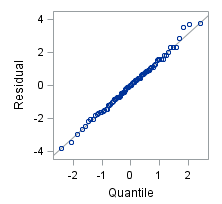
\includegraphics{normqq4c}

\item %4d

There is slightly less variation in the residuals from the PEMF1hr/day treatment and the PEMF3hr/day treatment groups, which is particularly noticeable in the PEMF3hr/day treatment group. The variances appear similar enough that the slightly less variable group may be due to random chance and is likely not a concern in terms of the accuracy of ANOVA results interpretations.

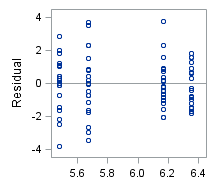
\includegraphics{residpred4d}

\item %4e

Higher bone mineral densities are desirable. We are given responses of percent losses in bone mineral density. Bone mineral density is ideal, and so we would like to minimize the percent loss in bone mineral density.

We would like to do a lower tailed test for whether the percentage of BMD loss has decreased.

Using 90\% family-wise confidence intervals, there is no evidence that any of the PEMF treatments reduce the percentage of BMD loss when compared to SHAM.

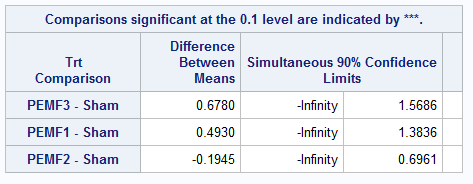
\includegraphics{prob4e}

\item %4f

At the 90\% confidence level, it is estimated that PEMF1hr/day caused percentage loss in BMD to be 1.3836\% or less on average than those receiving SHAM. The study description did not indicate random sampling, so inference was only made to ``those" in the study.
\end{enumerate}

\item 
\begin{enumerate}
\item 

$\Gamma_{L}$ = -1$\tau_{1hr}$ + 0$\tau_{2hr}$ + 1$\tau_{4hr}$

$\Gamma_{Q}$ = 1$\tau_{1hr}$ + -2$\tau_{2hr}$ + 1$\tau_{4hr}$

\item 

There was no evidence of the linear trend and some evidence of the quadratic trend. The boxplots are consistent with this as the median is slightly above 6 in the PEMF1 and PEMF3 (corresponds to PEMF4) treatments and slightly below 6 in the PEMF2 treatment.


\begin{center}
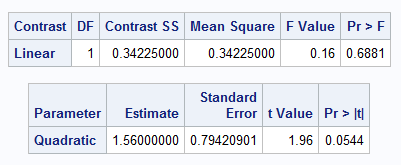
\includegraphics{prob2g1}
\end{center}

\begin{center}
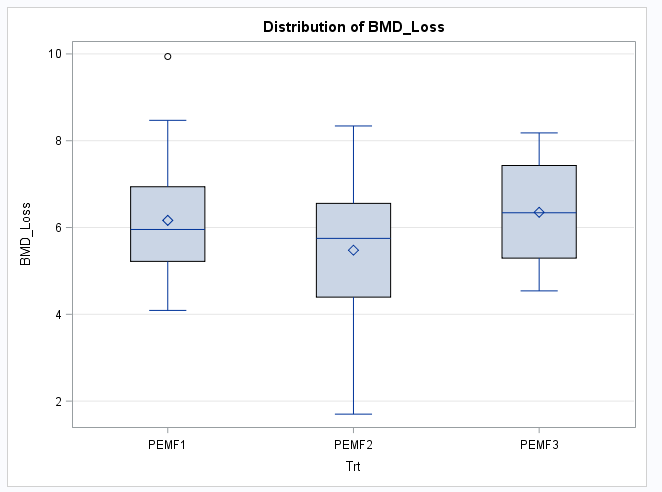
\includegraphics[scale=0.5]{boxplots1}
\end{center}

\item 

If I had used all treatment groups in the analysis, $SS_{L} + SS_{Q} \neq SS_{trt}$ because there are four treatment groups, we would need to add $SS_{cubic}$ to the linear and quadratic SS as that will completely partition the $SS_{trt}$. However, I omitted the SHAM group from the analysis so the mathematical statement $SS_{L} + SS_{Q} = SS_{trt}$ should be true as there are 3 treatment groups and therefore we can fit up to an order of 2 polynomial model.
\end{enumerate}
\item %5

Yes, there is a problem. Using the coefficients for the contrasts that were given in the notes we have to have equally spaced increments of treatments if the treatments are on the continuous scale and we are performing tests of linear and quadratic orthoganol contrasts. In this problem, the treatment increments are on the continuous scale and are not equally spaced.

A side question: Does the order of categorical treatments matter for these coefficients? In problem (4) we treated going from PEMF1hr/day to PEMF2hr/day as the same increment as PEMF2hr/day to PEMF4hr/day when doing the orthoganol trend contrasts, which may not be correct in that case unless that assumption is reasonable. Is that correct?

\item %6

\begin{enumerate}

\item %6a



The selected transformation was $\lambda$ = 0. Therefore, we should log the response to stabilize the variance. 

\begin{center}
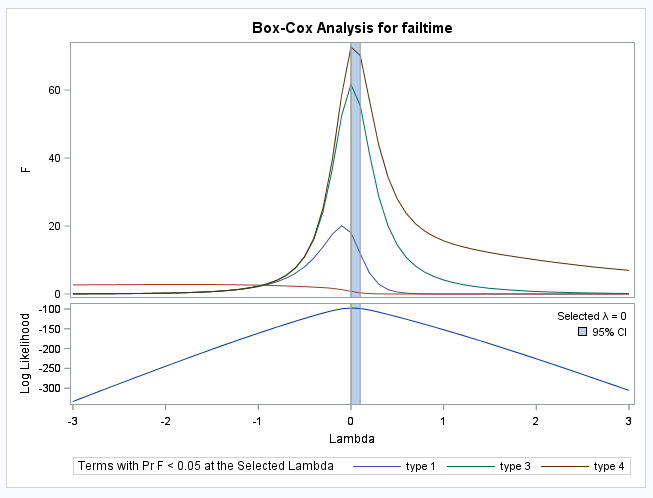
\includegraphics[scale=0.5]{prob6}

\end{center}

\item %6b

Normality is reasonable, however, of major concern is the violation of homogeneity of variance as one group has much less variable residuals than the others. The p-values from the ANOVA will be too small and we will find significant differences more often than we would expect if the HOV assumption was met.

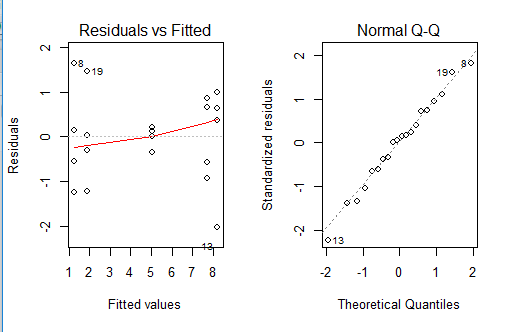
\includegraphics[scale=0.7]{prob6plots}

\begin{kframe}
\begin{alltt}
\hlstd{mat} \hlkwb{<-} \hlkwd{read.csv}\hlstd{(}\hlstr{"material.csv"}\hlstd{)}
\hlstd{mat}\hlopt{$}\hlstd{failtime.ln} \hlkwb{<-} \hlkwd{log}\hlstd{(mat}\hlopt{$}\hlstd{failtime)}

\hlstd{mat.mean} \hlkwb{<-} \hlkwd{tapply}\hlstd{(mat}\hlopt{$}\hlstd{failtime.ln,} \hlkwd{as.factor}\hlstd{(mat}\hlopt{$}\hlstd{type),mean)}
\hlstd{mat.s} \hlkwb{<-} \hlkwd{data.frame}\hlstd{((}\hlkwd{tapply}\hlstd{(mat}\hlopt{$}\hlstd{failtime.ln,} \hlkwd{as.factor}\hlstd{(mat}\hlopt{$}\hlstd{type),var)))}
\hlkwd{colnames}\hlstd{(mat.s)} \hlkwb{<-} \hlstr{"Sample Var"}
\hlkwd{rownames}\hlstd{(mat.s)} \hlkwb{<-} \hlkwd{c}\hlstd{(}\hlstr{"1"}\hlstd{,} \hlstr{"2"}\hlstd{,} \hlstr{"3"}\hlstd{,} \hlstr{"4"}\hlstd{,} \hlstr{"5"}\hlstd{)}

\hlkwd{print}\hlstd{(}\hlkwd{xtable}\hlstd{(mat.s))}
\end{alltt}
\end{kframe}% latex table generated in R 3.3.2 by xtable 1.8-2 package
% Fri Feb 10 08:54:09 2017
\begin{table}[ht]
\centering
\begin{tabular}{rr}
  \hline
 & Sample Var \\ 
  \hline
1 & 0.06 \\ 
  2 & 1.53 \\ 
  3 & 0.79 \\ 
  4 & 1.86 \\ 
  5 & 1.23 \\ 
   \hline
\end{tabular}
\end{table}
\begin{kframe}\begin{alltt}
\hlstd{lm1} \hlkwb{<-} \hlkwd{lm}\hlstd{(failtime.ln}\hlopt{~}\hlkwd{as.factor}\hlstd{(type),} \hlkwc{data} \hlstd{= mat)}

\hlkwd{par}\hlstd{(}\hlkwc{mfrow}\hlstd{=}\hlkwd{c}\hlstd{(}\hlnum{2}\hlstd{,}\hlnum{2}\hlstd{))}
\hlcom{#plot(lm1)}
\end{alltt}
\end{kframe}



\item %6c

Based on an $F_{4,15}$ = 37.657 and a p-value of $<$ 0.001 there is strong evidence that one of the material types has a different mean failure time than the others.
\begin{knitrout}\footnotesize
\definecolor{shadecolor}{rgb}{0.969, 0.969, 0.969}\color{fgcolor}\begin{kframe}
\begin{alltt}
\hlkwd{summary}\hlstd{(lm1)}
\end{alltt}
\begin{verbatim}

Call:
lm(formula = failtime.ln ~ as.factor(type), data = mat)

Residuals:
     Min       1Q   Median       3Q      Max 
-2.00945 -0.55716  0.08608  0.64969  1.64792 

Coefficients:
                 Estimate Std. Error t value Pr(>|t|)
(Intercept)        5.0516     0.5234   9.651 7.95e-08
as.factor(type)2  -3.8091     0.7402  -5.146 0.000119
as.factor(type)3   2.6648     0.7402   3.600 0.002625
as.factor(type)4   3.1624     0.7402   4.272 0.000668
as.factor(type)5  -3.1476     0.7402  -4.252 0.000695

Residual standard error: 1.047 on 15 degrees of freedom
Multiple R-squared:  0.9094,	Adjusted R-squared:  0.8853 
F-statistic: 37.66 on 4 and 15 DF,  p-value: 1.176e-07
\end{verbatim}
\begin{alltt}
\hlkwd{anova}\hlstd{(lm1)}
\end{alltt}
\begin{verbatim}
Analysis of Variance Table

Response: failtime.ln
                Df  Sum Sq Mean Sq F value    Pr(>F)
as.factor(type)  4 165.056  41.264  37.657 1.176e-07
Residuals       15  16.437   1.096                  
\end{verbatim}
\end{kframe}
\end{knitrout}

\end{enumerate}

\item %7

Below we see in the table that the means increase from a to c, however, the 95\% bonferroni adjusted CI for a-b is completely below zero and the 95\% bonferroni adjusted CI for a-c contains zero. These would correspond to rejecting the null of no difference and failing to reject the null of no difference respectively.

\begin{kframe}
\begin{alltt}
\hlkwd{set.seed}\hlstd{(}\hlnum{7}\hlstd{)}
\hlstd{a} \hlkwb{<-} \hlkwd{rnorm}\hlstd{(}\hlnum{100}\hlstd{,}\hlnum{10}\hlstd{,}\hlnum{5}\hlstd{)}
\hlstd{b} \hlkwb{<-} \hlkwd{rnorm}\hlstd{(}\hlnum{1000}\hlstd{,} \hlnum{14}\hlstd{,} \hlnum{10}\hlstd{)}
\hlstd{c} \hlkwb{<-} \hlkwd{rnorm}\hlstd{(}\hlnum{5}\hlstd{,}\hlnum{12}\hlstd{,}\hlnum{5}\hlstd{)}

\hlstd{dat} \hlkwb{<-} \hlkwd{data.frame}\hlstd{(}\hlkwd{matrix}\hlstd{(}\hlnum{0}\hlstd{,}\hlkwc{nrow}\hlstd{=}\hlkwd{length}\hlstd{(}\hlkwd{c}\hlstd{(a,b,c)),} \hlkwc{ncol} \hlstd{=} \hlnum{2}\hlstd{))}
\hlstd{dat}\hlopt{$}\hlstd{norm} \hlkwb{<-} \hlkwd{c}\hlstd{(a,b,c)}
\hlstd{dat}\hlopt{$}\hlstd{group} \hlkwb{<-} \hlkwd{c}\hlstd{(}\hlkwd{rep}\hlstd{(}\hlstr{"a"}\hlstd{,}\hlkwd{length}\hlstd{(a)),} \hlkwd{rep}\hlstd{(}\hlstr{"b"}\hlstd{,} \hlkwd{length}\hlstd{(b)),} \hlkwd{rep}\hlstd{(}\hlstr{"c"}\hlstd{,}\hlkwd{length}\hlstd{(c)))}
\hlstd{dat} \hlkwb{<-} \hlkwd{data.frame}\hlstd{(dat)}

\hlstd{lm.dat} \hlkwb{<-} \hlkwd{lm}\hlstd{(norm}\hlopt{~}\hlkwd{as.factor}\hlstd{(group),} \hlkwc{data} \hlstd{= dat)}
\hlcom{#summary(lm.dat)}

\hlkwd{write.csv}\hlstd{(dat,} \hlkwc{file} \hlstd{=} \hlstr{"prob7.csv"}\hlstd{)}

\hlstd{tb} \hlkwb{<-} \hlkwd{c}\hlstd{(}\hlkwd{mean}\hlstd{(a),} \hlkwd{mean}\hlstd{(b),} \hlkwd{mean}\hlstd{(c))}
\hlstd{tb} \hlkwb{<-} \hlkwd{data.frame}\hlstd{(tb)}

\hlkwd{rownames}\hlstd{(tb)} \hlkwb{<-} \hlkwd{c}\hlstd{(}\hlstr{"a"}\hlstd{,} \hlstr{"b"}\hlstd{,} \hlstr{"c"}\hlstd{)}
\hlkwd{colnames}\hlstd{(tb)} \hlkwb{<-} \hlkwd{c}\hlstd{(}\hlstr{"means"}\hlstd{)}

\hlkwd{print}\hlstd{(}\hlkwd{xtable}\hlstd{(tb,} \hlkwc{align} \hlstd{=} \hlstr{"||l|l||"}\hlstd{))}
\end{alltt}
\end{kframe}% latex table generated in R 3.3.2 by xtable 1.8-2 package
% Fri Feb 10 08:54:09 2017
\begin{table}[ht]
\centering
\begin{tabular}{||l|l||}
  \hline
 & means \\ 
  \hline
a & 10.69 \\ 
  b & 13.77 \\ 
  c & 20.61 \\ 
   \hline
\end{tabular}
\end{table}




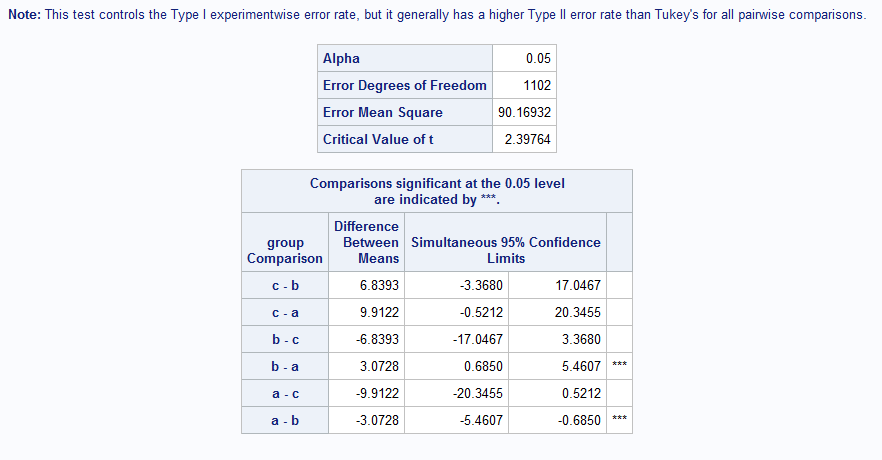
\includegraphics[scale=0.5]{prob7}



\end{enumerate}
\end{document}
